\documentclass[tikz,border=2pt]{standalone}
\usepackage{amsmath}
\begin{document}
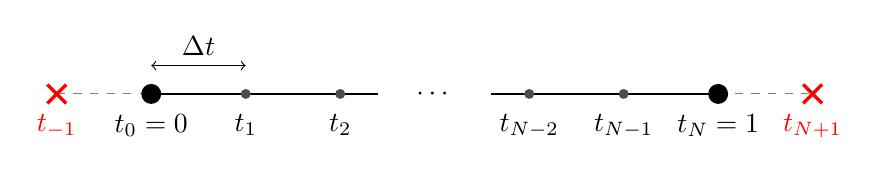
\begin{tikzpicture}[scale=1.2,
    cross/.style={red, line width=1.2pt},
    ]
    % axis line (dashed outside [0,1])
    \draw[dashed, gray] (-1,0) -- (0,0);
    \draw[dashed, gray] (6,0) -- (7,0);
    \draw[thick] (0,0) -- (2.4,0);
    \draw[thick] (3.6,0) -- (6,0);
    \node at (3,0) {$\cdots$};
    % interior points
    \foreach \x in {1,2,4,5} {
        \fill[gray!60!black] (\x,0) circle (1.5pt);
    }
    % boundary points
    \fill[black] (0,0) circle (3pt);
    \fill[black] (6,0) circle (3pt);
    % ghost points
    \foreach \x in {-1,7} {
        \draw[cross] (\x-0.1,-0.1) -- (\x+0.1,0.1);
        \draw[cross] (\x-0.1,0.1) -- (\x+0.1,-0.1);
    }
    % labels
    \node[below=4pt, red] at (-1,0) {$t_{-1}$};
    \node[below=4pt] at (0,0) {$t_0 = 0$};
    \node[below=4pt] at (1,0) {$t_1$};
    \node[below=4pt] at (2,0) {$t_2$};
    \node[below=4pt] at (4,0) {$t_{N-2}$};
    \node[below=4pt] at (5,0) {$t_{N-1}$};
    \node[below=4pt] at (6,0) {$t_N = 1$};
    \node[below=4pt, red] at (7,0) {$t_{N+1}$};
    % grid spacing
    \draw[<->] (0,0.3) -- node[above] {$\Delta t$} (1,0.3);
\end{tikzpicture}
\end{document}
